\chapter{Literature Review and Theoretical Background}
\label{ch:literature}

This chapter establishes the theoretical foundation for the CHOYXONA.UZ project.
It traces the evolution of mobile application development, analyzes existing restaurant booking platforms, examines the Flutter framework and Firebase backend services selected for implementation, and articulates the research motivation and direction.


% =====================================================================
\section{Core Concepts and Definitions}
\label{sec:core-concepts}

Before analyzing technologies and platforms, it is essential to define the key concepts used throughout this thesis.

\textbf{Cross-platform mobile development} refers to the practice of building mobile applications that run on multiple operating systems (primarily iOS and Android) from a single shared codebase, as opposed to native development which requires separate codebases for each platform~\cite{elkassas2017}.
This approach reduces development time and maintenance costs while enabling broader market reach.

\textbf{Backend-as-a-Service (BaaS)} is a cloud computing model that provides developers with pre-built server-side functionality including authentication, database management, file storage, and push notifications, eliminating the need to build and maintain custom server infrastructure~\cite{moroney2017}.

\textbf{Real-time synchronization} describes the capability of a system to propagate data changes from the server to all connected clients immediately, without requiring explicit refresh actions.
In the context of booking applications, this ensures that availability information displayed to users reflects the current state of reservations~\cite{firebase_firestore2024}.

\textbf{Restaurant booking system} (or reservation management system) is a software platform that enables customers to discover dining establishments, view availability, and make reservations electronically, while providing establishment operators with tools for managing bookings, analyzing performance, and communicating with customers~\cite{opentable2023}.

\textbf{Choyxona} (also transliterated as ``chayhana'' or ``chaikhana'') is a traditional Central Asian teahouse serving as a social gathering place where food and tea are served.
In Uzbekistan, choyxonas feature private rooms (``xona'') for family gatherings, celebrations, and business meetings, distinguishing them from typical Western restaurant formats.


% =====================================================================
\section{Evolution of Mobile Application Development}
\label{sec:mobile-evolution}

The mobile application industry has undergone remarkable transformation since the introduction of the first smartphone applications in the late 2000s.
The launch of Apple's App Store in July 2008 and Google Play (initially called Android Market) in October 2008 established the foundation for a global ecosystem that now encompasses millions of applications serving billions of users worldwide~\cite{statista2024}.

The evolution of mobile development can be characterized by three distinct phases, each marked by technological advances and shifting developer preferences, as illustrated in \cref{fig:mobile-evolution}.

\begin{figure}[htbp]
  \centering
  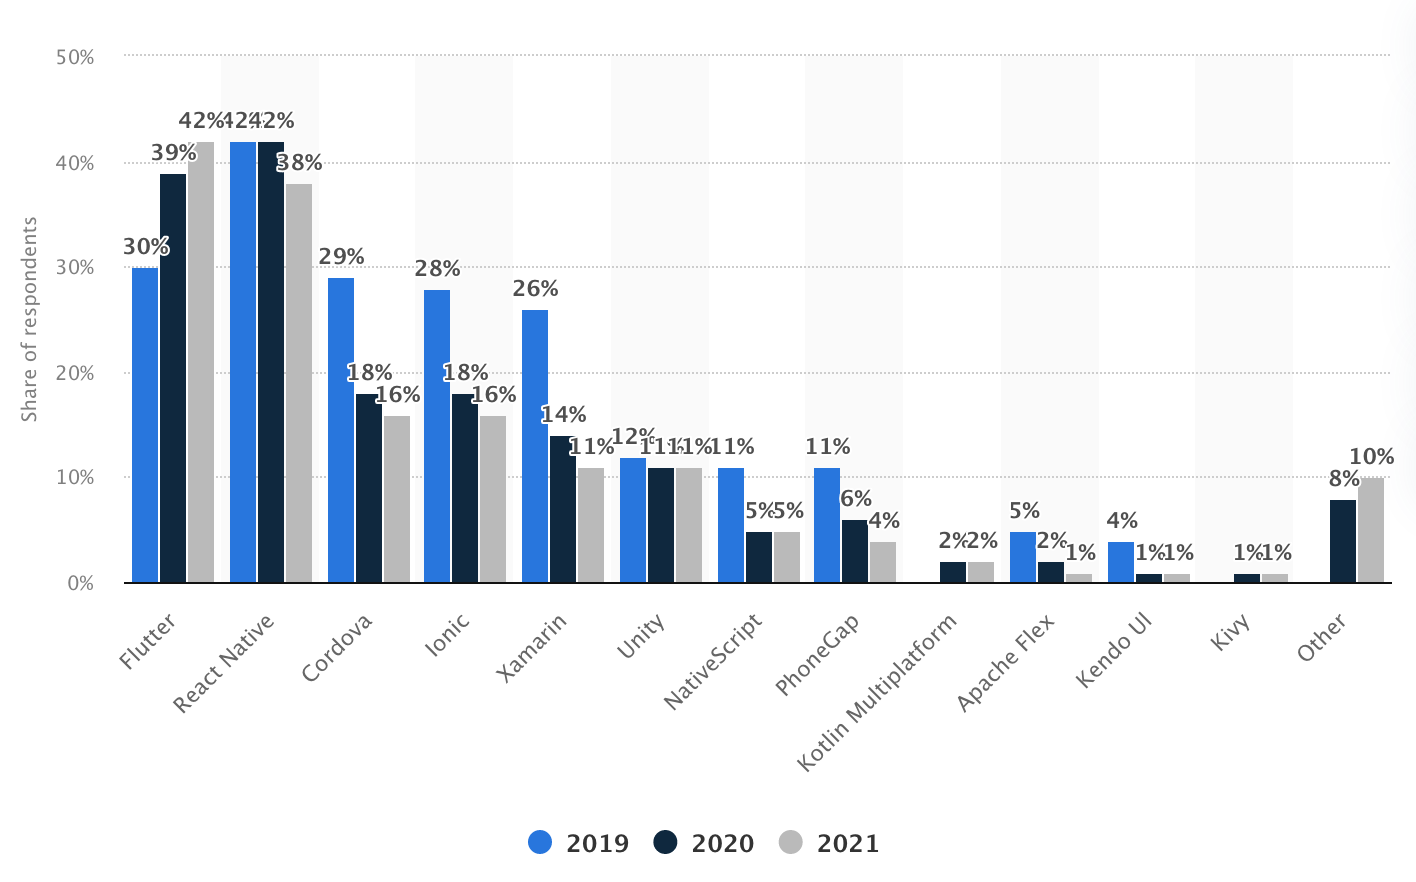
\includegraphics[width=0.85\textwidth]{b_chapters/chapter1/assets/f-1.png}
  \figsource{Author-created illustration based on industry timeline analysis.}
  \caption{Evolution of mobile application development frameworks (2008--2025).}
  \label{fig:mobile-evolution}
\end{figure}

\textbf{Phase~1: Native dominance (2008--2012).}
The first phase was dominated by native development approaches.
Developers created separate codebases for iOS using Objective-C and for Android using Java.
This approach required specialized expertise for each platform and resulted in high development costs, as essentially two complete applications needed to be built and maintained.
The advantages of native development included optimal performance and full access to platform-specific features, but the resource requirements limited this approach to well-funded organizations~\cite{charland2011}.

\textbf{Phase~2: Hybrid emergence (2012--2016).}
The second phase witnessed the emergence of hybrid frameworks designed to address the cost and complexity challenges of native development.
Technologies such as Apache Cordova (PhoneGap) allowed developers to write applications using web technologies (HTML, CSS, JavaScript) and package them for multiple platforms.
Ionic Framework built upon Cordova to provide pre-built UI components.
React Native, released by Facebook in 2015, introduced a different approach using native components rather than web views~\cite{biorn2017}.
These technologies promised write-once-deploy-everywhere capability but often suffered from performance limitations and inconsistent user experiences~\cite{lim2015}.

\textbf{Phase~3: Near-native cross-platform (2017--present).}
The current phase is characterized by sophisticated cross-platform frameworks achieving near-native performance while maintaining the single-codebase advantage.
Flutter, released by Google in May 2017 and reaching stable version~1.0 in December 2018, represents a significant advancement.
Unlike predecessors, Flutter compiles to native ARM code and renders its own widgets using the Skia graphics engine, achieving consistent visual appearance and 60~fps animations on standard devices~\cite{flutter_arch2024}.

The global mobile application market has demonstrated consistent growth throughout this evolution.
According to Statista, mobile app downloads worldwide reached 255~billion in 2022, with revenue exceeding 430~billion~USD~\cite{statista2024}.
In Uzbekistan, internet penetration reached approximately 77\% in 2023, with mobile devices accounting for the majority of internet access.
The success of local mobile payment applications such as Click and Payme demonstrates that Uzbek consumers are ready to adopt mobile solutions that provide genuine value~\cite{gartner2023}.


% =====================================================================
\section{Analysis of Online Booking Systems}
\label{sec:booking-analysis}

The restaurant booking industry has evolved from simple telephone reservation systems to sophisticated platforms offering comprehensive hospitality solutions.
Understanding existing platforms provides valuable context for the development of CHOYXONA.UZ and helps identify both successful patterns and gaps that remain unaddressed in certain markets.

\textbf{OpenTable}, founded in 1998, pioneered online restaurant reservations and remains one of the largest platforms globally.
Acquired by Booking Holdings in 2014 for approximately 2.6~billion~USD, OpenTable serves over 60,000 restaurants with a comprehensive reservation management system including floor management, guest profiles, analytics dashboards, and POS integration.
Revenue comes from monthly subscription fees and per-cover charges~\cite{opentable2023}.

\textbf{TheFork}, a TripAdvisor company, demonstrates the importance of integration with review ecosystems.
By combining reservation functionality with millions of TripAdvisor reviews, TheFork provides discovery-to-booking experiences primarily in European markets.
Its \enquote{Yums} loyalty program incentivizes repeat bookings~\cite{gartner2023}.

\textbf{Resy}, founded in 2014 and acquired by American Express in 2019, targets the high-end dining segment with exclusive access to sought-after reservations.
Integration with American Express card benefits provides priority access, highlighting natural synergies between dining reservations and payment ecosystems.

\textbf{Yelp Reservations} demonstrates how discovery platforms naturally extend into transactional functionality.
Yelp's strength in user-generated reviews and local search makes it significant in the restaurant discovery journey, even when actual booking transactions occur through partner services~\cite{nielsen2012}.

A comparative analysis of these platforms reveals several common success factors, summarized in \cref{tab:platform-comparison}.

\begin{table}[htbp]
\caption{Comparison of global restaurant booking platforms}
\label{tab:platform-comparison}
\centering
\small
\begin{tabular}{lcccc}
\toprule
\textbf{Feature} & \textbf{OpenTable} & \textbf{TheFork} & \textbf{Resy} & \textbf{Yelp} \\
\midrule
Two-sided marketplace  & \checkmark & \checkmark & \checkmark & \checkmark \\
Review \& rating system & \checkmark & \checkmark & Partial    & \checkmark \\
Loyalty program         & ---        & \checkmark & \checkmark & ---        \\
POS integration         & \checkmark & Partial    & \checkmark & ---        \\
Mobile app              & \checkmark & \checkmark & \checkmark & \checkmark \\
Private room booking    & Partial    & ---        & ---        & ---        \\
Central Asian coverage  & ---        & ---        & ---        & ---        \\
Multilingual (UZ/RU/EN) & ---        & ---        & ---        & ---        \\
\bottomrule
\end{tabular}
\end{table}

As \cref{tab:platform-comparison} demonstrates, none of the major platforms provide Central Asian market coverage or support for Uzbek and Russian languages.
Furthermore, the private room booking capability essential for choyxona culture is either absent or only partially supported.
The Central Asian market presents unique characteristics that differentiate it from Western markets: teahouses feature private rooms for extended gatherings lasting several hours, cultural preferences regarding hospitality create specific requirements, and menu offerings center around traditional cuisine with specific preparation requirements~\cite{gartner2023}.

\begin{figure}[htbp]
  \centering
  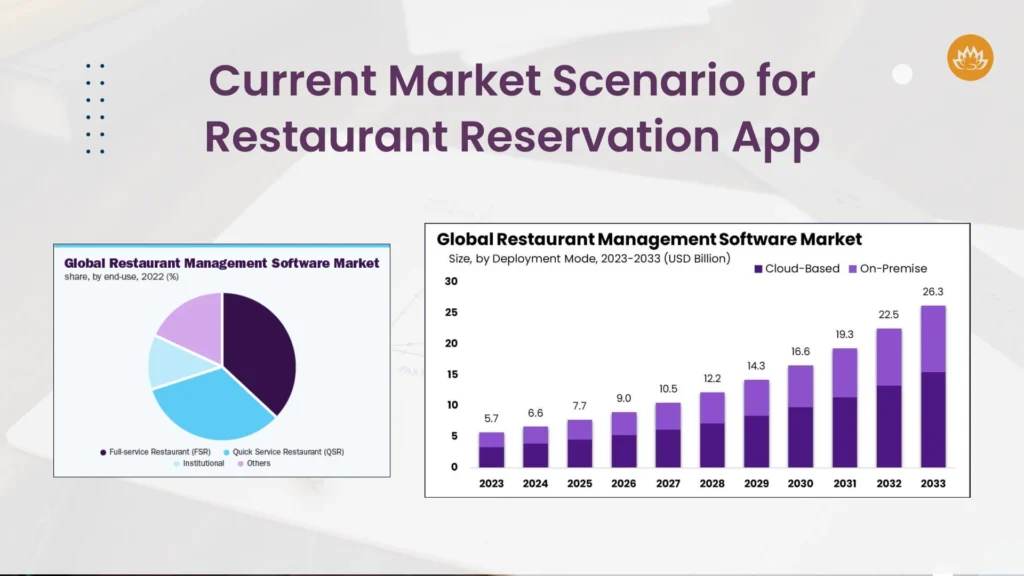
\includegraphics[width=0.7\textwidth]{b_chapters/chapter1/assets/f-2.png}
  \figsource{Author-created illustration based on platform analysis.}
  \caption{Feature coverage analysis of global booking platforms vs. Uzbek market requirements.}
  \label{fig:platform-gap}
\end{figure}

The competitive landscape in Uzbekistan for restaurant booking is currently limited.
While general business directories and social media pages provide some discovery functionality, no dedicated booking platform with real-time availability and confirmation has achieved significant adoption.
This gap validates the opportunity for CHOYXONA.UZ to establish market leadership with a culturally adapted solution.


% =====================================================================
\section{Flutter Framework: Architecture and Advantages}
\label{sec:flutter}

Flutter is an open-source user interface software development kit created by Google that enables developers to build natively compiled applications for mobile, web, and desktop platforms from a single codebase written in the Dart programming language.
Since its initial stable release in December 2018, Flutter has grown rapidly, with Google reporting over 3~million developers using the framework by 2022~\cite{flutter_arch2024}.

The architecture of Flutter differs fundamentally from other cross-platform solutions, as illustrated in \cref{fig:flutter-arch}.
While frameworks like React Native bridge JavaScript code to native components through a middleware layer, Flutter maintains its own rendering engine based on Skia --- the same graphics library used by Google Chrome and Android.
Rather than wrapping or bridging to platform-specific components, Flutter draws every pixel of the user interface directly using its own rendering pipeline~\cite{windmill2020}.

\begin{figure}[htbp]
  \centering
  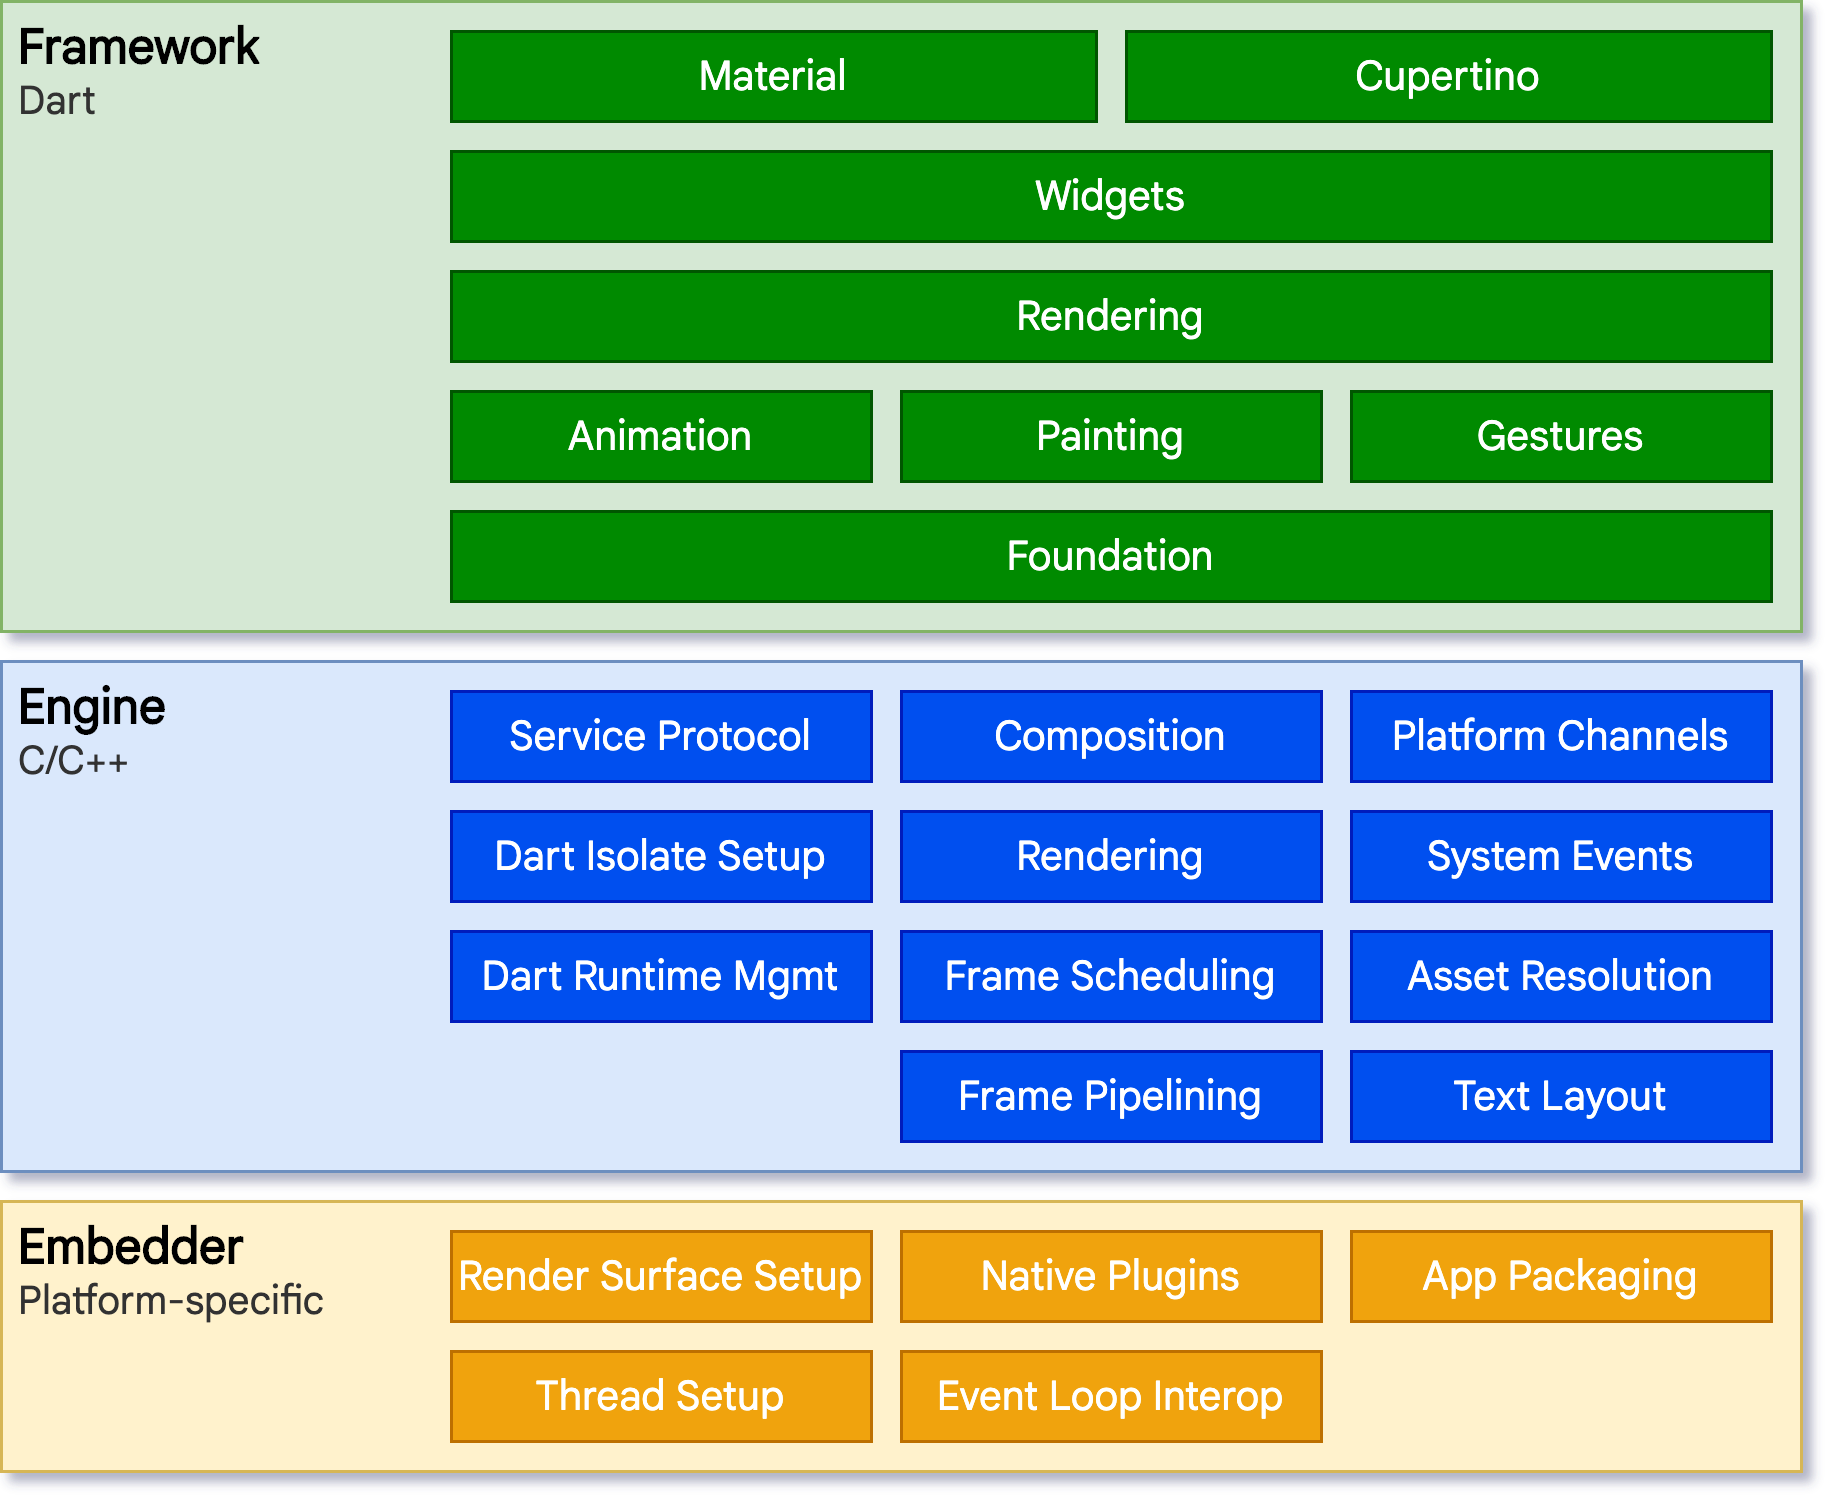
\includegraphics[width=0.75\textwidth]{b_chapters/chapter1/assets/f-3.png}
  \figsource{Adapted from Flutter official documentation~\cite{flutter_arch2024}.}
  \caption{Flutter framework architecture and rendering pipeline.}
  \label{fig:flutter-arch}
\end{figure}

This architecture provides several significant advantages:
\begin{itemize}
  \item \textbf{Visual consistency} across platforms, since the same rendering code executes on both iOS and Android.
  \item \textbf{Fine-grained pixel control}, enabling precise implementation of custom designs.
  \item \textbf{High-performance animations} at 60~fps on standard devices and 120~fps on high-refresh-rate displays.
  \item \textbf{Hot reload} capability reflecting code changes within milliseconds during development, transforming the iteration experience~\cite{napoli2021}.
\end{itemize}

The \textbf{Dart programming language}, created by Google, provides features well-suited for UI programming: compilation to native ARM code for performance, both ahead-of-time and just-in-time compilation, strong static typing with type inference, null safety (since Dart~2.12), and asynchronous programming support through futures and streams~\cite{dart2024}.

Flutter's \textbf{widget-based architecture} organizes the user interface as a tree of immutable widget objects.
Everything in Flutter is a widget --- from structural elements like rows and columns to interactive elements like buttons and text fields.
When application state changes, Flutter rebuilds the affected portion of the widget tree and efficiently updates only the changed portions of the rendering tree.
This declarative approach simplifies UI development and reduces bugs associated with manually managing view updates~\cite{payne2019}.

\textbf{State management} represents a critical architectural decision.
The Provider package, officially recommended by the Flutter team, implements the InheritedWidget pattern for efficient state sharing.
Alternative approaches include BLoC (Business Logic Component) using streams, Riverpod with improved error handling, and GetX prioritizing developer convenience~\cite{flutter_state2024}.
CHOYXONA.UZ employs Provider for state management, balancing simplicity with sufficient capability.

A comparative analysis of cross-platform frameworks informed the technology selection, as summarized in \cref{tab:framework-comparison}.

\begin{table}[htbp]
\caption{Comparison of cross-platform mobile development frameworks}
\label{tab:framework-comparison}
\centering
\small
\begin{tabular}{lccc}
\toprule
\textbf{Criterion} & \textbf{Flutter} & \textbf{React Native} & \textbf{Kotlin MP} \\
\midrule
Language              & Dart         & JavaScript/TS   & Kotlin       \\
Rendering             & Own engine   & Native bridge   & Native UI    \\
Performance           & Near-native  & Good            & Native       \\
UI consistency        & Excellent    & Platform-dependent & Platform-native \\
Hot reload            & \checkmark   & \checkmark      & Partial      \\
Single codebase       & \checkmark   & \checkmark      & Logic only   \\
Community size        & Large        & Very large      & Growing      \\
Desktop/Web support   & \checkmark   & Limited         & Experimental \\
Google backing        & \checkmark   & Meta            & JetBrains    \\
Null safety           & \checkmark   & TypeScript      & \checkmark   \\
\bottomrule
\end{tabular}
\end{table}

Flutter was selected for CHOYXONA.UZ based on alignment with project requirements: the single codebase approach matched resource constraints, the modern Dart language reduces runtime errors, the extensive widget library provides pre-built Material Design components, and Google's continued investment ensures long-term viability~\cite{wu2018, xanthopoulos2013}.


% =====================================================================
\section{Firebase Backend-as-a-Service}
\label{sec:firebase}

Firebase is a comprehensive application development platform provided by Google, offering a suite of services that accelerate development by handling common backend requirements.
Originally founded as an independent company in 2011 focused on real-time database functionality, Firebase was acquired by Google in 2014 and has expanded to include authentication, hosting, cloud functions, analytics, and numerous other services~\cite{moroney2017}.
The Firebase services architecture relevant to CHOYXONA.UZ is presented in \cref{fig:firebase-services}.

\begin{figure}[htbp]
  \centering
  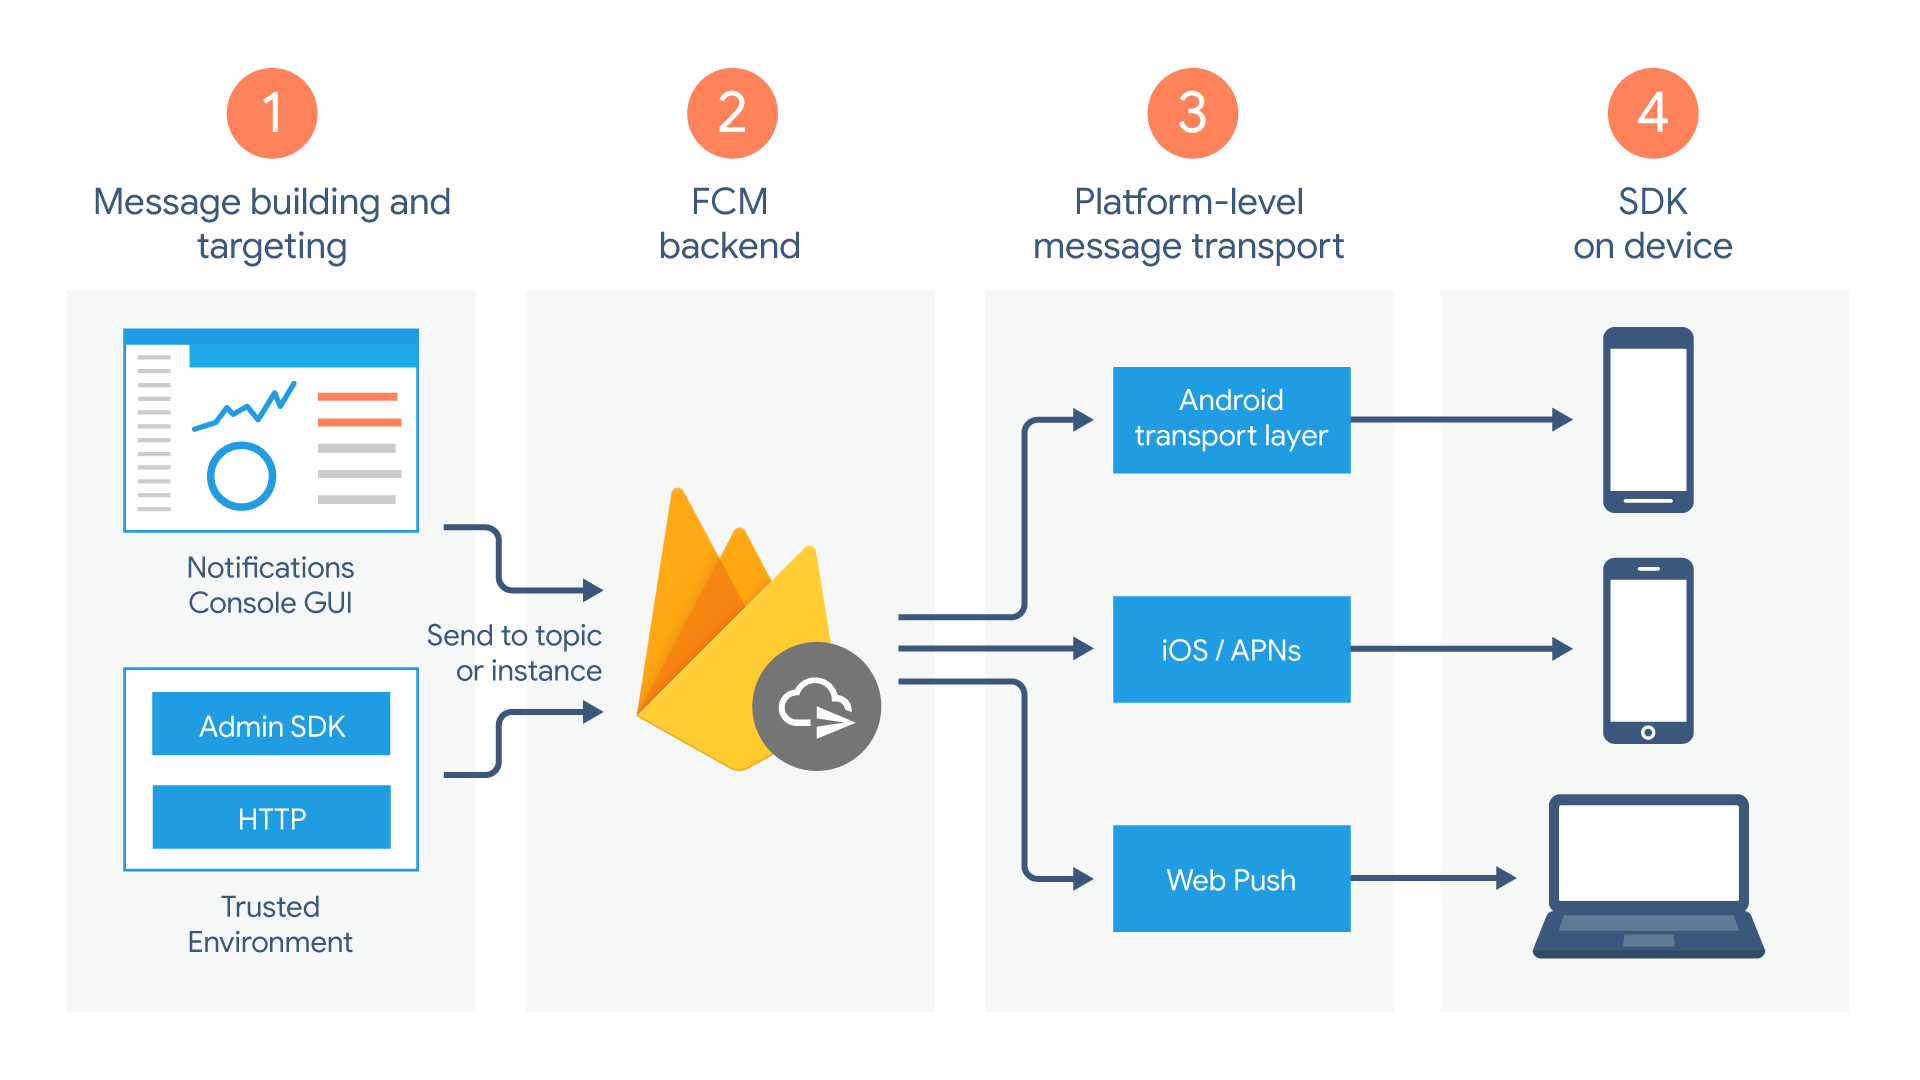
\includegraphics[width=0.75\textwidth]{b_chapters/chapter1/assets/f-4.png}
  \figsource{Author-created illustration based on Firebase documentation~\cite{firebase_auth2024}.}
  \caption{Firebase services architecture used in the CHOYXONA.UZ application.}
  \label{fig:firebase-services}
\end{figure}

\textbf{Firebase Authentication} supports multiple sign-in methods.
For CHOYXONA.UZ, email/password and phone number (SMS) authentication were implemented, aligning with user expectations in Uzbekistan where phone numbers serve as primary identifiers.
The service handles secure password hashing, session management, brute-force protection, and account recovery~\cite{firebase_auth2024}.

\textbf{Cloud Firestore} serves as the primary database, providing flexible, scalable NoSQL document storage with real-time synchronization capabilities.
Unlike traditional SQL databases with fixed schemas, Firestore stores data in collections of documents containing key-value pairs and subcollections for hierarchical organization.
The real-time synchronization capability enables Firestore clients to subscribe to document snapshots, receiving automatic updates through persistent connections whenever data changes on the server~\cite{firebase_firestore2024}.
This capability is particularly valuable for booking applications where availability can change rapidly.

\textbf{Firebase Cloud Storage} provides secure file storage for user-generated content including profile photos, establishment images, and menu item photos.
Storage security rules reference the authenticated user's identity, enabling patterns such as allowing users to upload their own profile photos while preventing modification of others' files~\cite{moroney2017}.

\textbf{Firebase Cloud Messaging (FCM)} enables push notifications on both Android and iOS platforms.
CHOYXONA.UZ uses FCM for booking confirmations, reservation reminders (24~hours and 2~hours before), promotional notifications from establishments, and system announcements.
The notification system reaches users even when the application is not actively running~\cite{firebase_functions2024}.

The \textbf{pricing model} follows a usage-based approach with generous free tiers.
The free Spark plan includes 1~GiB Firestore storage, 10~GiB Cloud Storage, and 50,000 daily active users for Authentication.
The Blaze plan charges based on actual usage, reducing initial infrastructure investment while providing a clear scaling path~\cite{khawas2018}.

\textbf{Security Rules} enforce authorization declaratively at the database level.
Rules execute on Firebase servers, ensuring enforcement regardless of client behavior.
CHOYXONA.UZ implements role-based access control: regular users can only read their own bookings, administrators manage their own establishment, and super administrators have broader platform access~\cite{firebase_firestore2024}.

The integration of Firebase services into the Flutter application leverages official packages maintained by the \textbf{FlutterFire} project: \texttt{firebase\_core} for initialization, \texttt{firebase\_auth} for authentication, \texttt{cloud\_firestore} for database access, \texttt{firebase\_storage} for file management, and \texttt{firebase\_messaging} for push notifications~\cite{firebase_auth2024}.


% =====================================================================
\section{Research Motivation and Direction}
\label{sec:motivation}

\textbf{Problem significance.}
The analysis conducted in \cref{sec:booking-analysis} reveals that the Central Asian hospitality market remains unserved by major international booking platforms.
Uzbekistan, with over 35~million population and rapidly growing smartphone penetration, represents a significant addressable market.
Customers face difficulty discovering establishments matching their preferences, uncertainty about availability, and limited access to reviews.
Establishment owners lack tools for efficient booking management, customer analytics, and digital marketing~\cite{gartner2023}.

\textbf{Identified gap.}
From the comparison in \cref{sec:booking-analysis} and \cref{tab:platform-comparison}, the unmet need is clear: no existing platform provides a localized, culturally adapted booking solution that supports Uzbek teahouse conventions (private rooms, extended gatherings), multilingual interface (Uzbek, Russian, English), and real-time availability management tailored to the regional market.

\textbf{Direction and scope.}
This thesis pursues the development of CHOYXONA.UZ --- a complete cross-platform mobile application addressing the identified gap.
The scope encompasses:
\begin{itemize}
  \item Customer-facing features for discovery, search, and booking.
  \item Administrator tools for establishment management and analytics.
  \item Super administrator capabilities for platform oversight.
  \item Multi-platform deployment strategy for maximum market reach.
\end{itemize}
Deliberately out of scope for the initial release: integrated payment processing, AI-powered recommendations, and geographic expansion beyond Uzbekistan.

\textbf{Success criteria.}
The approach succeeds if: (1)~the application achieves acceptable performance metrics (cold start under 3~seconds, 60~fps scrolling, sub-200~ms query latency); (2)~successful deployment to Google Play, App Store, and alternative marketplaces; (3)~positive user acceptance testing results validating usability across target personas.


% =====================================================================
\section{Chapter Summary}
\label{sec:ch1-summary}

This chapter established the theoretical and analytical foundation for the CHOYXONA.UZ project through four key contributions:

First, \cref{sec:core-concepts} defined the conceptual vocabulary including cross-platform development, BaaS, real-time synchronization, and the choyxona cultural context that governs application requirements.

Second, \cref{sec:mobile-evolution} traced the evolution of mobile development through three phases --- native dominance, hybrid emergence, and near-native cross-platform --- demonstrating that modern frameworks like Flutter have matured to a point where single-codebase development no longer requires significant performance or quality compromises.

Third, \cref{sec:booking-analysis} conducted a comparative analysis of major booking platforms (OpenTable, TheFork, Resy, Yelp), identifying that while these platforms successfully serve Western markets, none provide coverage for Central Asia, support for Uzbek/Russian languages, or accommodation of choyxona-specific booking patterns such as private room reservations.

Fourth, \cref{sec:flutter,sec:firebase} justified the technology selection of Flutter and Firebase through systematic comparison with alternatives (\cref{tab:framework-comparison}), demonstrating alignment with project constraints including small team size, cross-platform requirements, real-time data needs, and cost-effective infrastructure.

Finally, \cref{sec:motivation} articulated the concrete research gap --- the absence of a localized, culturally adapted booking platform for Uzbekistan --- and defined measurable success criteria that will be evaluated in \cref{ch:testing}.

These analyses motivate the system architecture and design presented in Chapter~2 and the implementation described in Chapter~3.
